\documentclass{ctexart}
\usepackage{Note}
\begin{document}
\section{几何变换}
\subsection{几何变换基础}
\begin{theorem}[平移]
    平移对应的数学操作为向量加法.设物体上任意一点$P$的坐标为$\vec{p}$,平移向量为$\vec{t}$,则平移后的点$P'$的坐标$\vec{p}'=\vec{p}+\vec{t}$.例如,对于三维空间而言有
    \[\begin{bmatrix}
        x'\\y'\\z'
    \end{bmatrix}=\begin{bmatrix}
        x\\y\\z
    \end{bmatrix}+\begin{bmatrix}
        t_x\\t_y\\t_z
    \end{bmatrix}=\begin{bmatrix}
        x+t_x\\y+t_y\\z+t_z
    \end{bmatrix}\]
\end{theorem}
\begin{theorem}[旋转]
    旋转对应的数学操作为矩阵乘法.设物体上任意一点$P$的坐标为$\vec{p}$,旋转矩阵为$\mat{R}$,则旋转后的点$P'$的坐标$\vec{p}'=\mat{R}\vec{p}$.在二维平面中,绕原点逆时针旋转$\theta$角度的旋转矩阵为
    \[\mat{R}=\begin{bmatrix}
        \cos\theta & -\sin\theta\\
        \sin\theta & \cos\theta
    \end{bmatrix}\]
    在三维空间中,绕$x,y,z$轴分别旋转$\alpha,\beta,\gamma$角度的旋转矩阵分别为
    \[\mat{R}_x=\begin{bmatrix}
        1 & 0 & 0\\
        0 & \cos\alpha & -\sin\alpha\\
        0 & \sin\alpha & \cos\alpha
    \end{bmatrix},\quad \mat{R}_y=\begin{bmatrix}
        \cos\beta & 0 & \sin\beta\\
        0 & 1 & 0\\
        -\sin\beta & 0 & \cos\beta
    \end{bmatrix},\quad \mat{R}_z=\begin{bmatrix}
        \cos\gamma & -\sin\gamma & 0\\
        \sin\gamma & \cos\gamma & 0\\
        0 & 0 & 1
    \end{bmatrix}\]
\end{theorem}
\begin{theorem}[绕任意轴的旋转]
    在三维空间中,绕单位向量$\vec{a}=\left(a_x,a_y,a_z\right)$定义的轴逆时针旋转$\theta$角度的旋转矩阵$\mat{R}$为
    \[\mat{R}=\cos\theta\begin{bmatrix}
        1&0&0\\
        0&1&0\\
        0&0&1
    \end{bmatrix}+(1-\cos\theta)\begin{bmatrix}
        a_x^2 & a_xa_y & a_xa_z\\
        a_xa_y & a_y^2 & a_ya_z\\
        a_xa_z & a_ya_z & a_z^2
    \end{bmatrix}+\sin\theta\begin{bmatrix}
        0 & -a_z & a_y\\
        a_z & 0 & -a_x\\
        -a_y & a_x & 0
    \end{bmatrix}\]
\end{theorem}
\begin{proof}
    考虑三维空间中的点$\vec{v}$,旋转轴$\vec{a}$和旋转角度$\theta$.从$\vec{v}$旋转至$\vec{v}'$的操作可以分解为平行于$\vec{a}$的分量$\vec{r}$和垂直于$\vec{a}$的分量$\vec{u}$.\\
    根据投影向量的定义, $\vec{r}=(\vec{v}\cdot\vec{a})\vec{a}$, $\vec{u}=\vec{v}-(\vec{v}\cdot\vec{a})\vec{a}$.旋转过程中, $\vec{r}$保持不变,而$\vec{u}$则绕$\vec{a}$旋转$\theta$角度,这可以由下面的方式得到
    \[\vec{u}'=\vec{u}\cos\theta+\vec{u}^{\bot}\sin\theta\]
    注意到$\vec{u}^\bot=\vec{a}\times\vec{v}$,于是可得
    \[\begin{aligned}
        \vec{v}'
        &= \left[\left(\vec{v}-(\vec{v}\cdot\vec{a})\vec{a}\right)\cos\theta\right]+(\vec{a}\times\vec{v})\sin\theta+(\vec{v}\cdot\vec{a})\vec{a} \\
        &= \vec{v}\cos\theta+(1-\cos\theta)(\vec{v}\cdot\vec{a})\vec{a}+(\vec{a}\times\vec{v})\sin\theta
    \end{aligned}\]
    定义$\vec{a}$的反对称矩阵为
    \[\vec{a}^\ast=\begin{bmatrix}
        0 & -a_z & a_y\\
        a_z & 0 & -a_x\\
        -a_y & a_x & 0
    \end{bmatrix}\]
    不难根据矩阵乘法和向量叉乘的定义得出$\vec{a}\times\vec{v}=\vec{a}^\ast\vec{v}$.\\
    根据点积的定义有
    \[(\vec{a}\cdot\vec{x})\vec{a}=\left(\vec{a}^\t\vec{x}\right)\vec{a}=\vec{a}\left(\vec{a}^\t\vec{x}\right)=\left(\vec{a}\vec{a}^{\t}\right)\vec{x}\]
    于是将上述$\vec{v}'$的式子写作矩阵乘法即有
    \[\vec{v}'=\left[\mat{I}\cos\theta+\vec{a}\vec{a}^\t(1-\cos\theta)+\vec{a}^\ast\sin\theta\right]\vec{v}\]
    于是旋转矩阵即为
    \[\mat{R}=\mat{I}\cos\theta+\vec{a}\vec{a}^\t(1-\cos\theta)+\vec{a}^\ast\sin\theta\]
\end{proof}
\subsection{齐次坐标系及其中的几何变换}
我们在上一节中简单介绍了几何变换对应的数学操作.例如,平移可以视作向量的加法,旋转可以视作旋转矩阵与向量的乘法.但是,这些操作并不能统一表示,因而带来了额外的麻烦.例如,平移无法表示为矩阵与向量的乘法.为了解决这个问题,我们可以引入齐次坐标系的概念.
\subsubsection{齐次坐标系的定义}
\indent 齐次坐标系的基本思想是,通过引入额外的维度,将所有的几何变换都表示为矩阵与向量的乘法.
\begin{definition}[齐次坐标系]
    在$n$维空间$R^n$中,点$\vec{v}=\left(\li x,n\right)$的齐次坐标表示为$\left(\li x,n,1\right)$,即在原有坐标的基础上增加一个分量恒为$1$的维度.\\
    相应地,齐次坐标系中的向量$\vec{v}=\left(\li x,n\right)$表示为$\left(\li x,n,0\right)$,即在原有坐标的基础上增加一个分量恒为$0$的维度.
\end{definition}
如此,我们可以将所有的几何变换都表示为$(n+1)\times(n+1)$的矩阵与齐次坐标向量的乘法.
\subsubsection{齐次坐标系中几何变换的表示方式}
这里以三维空间为例介绍齐次坐标系中几何变换的表示方式.
\begin{theorem}[齐次坐标系中的平移矩阵]
    平移向量$\vec{t}=(t_x,t_y,t_z)$的平移矩阵为
    \[\mat{T}=\mat{I}+\begin{bmatrix}
        \vec{t}\\0
    \end{bmatrix}\]
    对于空间中任意一点$\vec{p}$,在齐次坐标系下总有
    \[\begin{bmatrix}
        \vec{p}+\vec{t}\\1
    \end{bmatrix}=\mat{T}\begin{bmatrix}
        \vec{p}\\1
    \end{bmatrix}\]
\end{theorem}
\begin{proof}
    简单地运用矩阵乘法的定义就能得到.
\end{proof}
\begin{theorem}[齐次坐标系中的旋转矩阵]
    齐次坐标系中的旋转矩阵为
    \[\mat{R}=\begin{bmatrix}
        \mat{R}'&\mbf0\\
        \mbf0&1
    \end{bmatrix}\]
    其中$\mat{R}'$为三维空间中的旋转矩阵,在前面已经推出其具体形式.
\end{theorem}
于是在齐次坐标系下,任何平移与旋转变换都可以写作矩阵
\[\begin{bmatrix}
    \mat{R}&\vec{t}\\\mbf0&1
\end{bmatrix}\]
与齐次坐标向量的乘法形式.
\subsection{几何变换在模型渲染中的应用}
对于渲染这一过程来说,将三维模型投影到二维平面上是一个重要的步骤.观察者的位置和视角决定了投影的结果.通常,我们需要观察者的位置$\vec{p}$,观察平面的法向量$\vec{n}$和视角正上方的方向$\vec{v}$决定.
\subsubsection{坐标变换}
\indent 在观察者的坐标中,$\vec{n}$通常指向$z$轴正方向,$\vec{v}$指向$y$轴正方向.而$x$轴方向根据左右手坐标系而确定.这里假定$x$轴的方向为$\vec{u}=\vec{v}\times\vec{n}$.因此,我们先需要把模型从世界坐标系$\mathcal{C}_{\text{world}}$变换到观察坐标系$\mathcal{C}_{\text{obs}}$上.
\paragraph{二维坐标变换}
为了研究坐标系变换问题,我们从二维坐标系变换开始.\\
\indent 考虑$\vec{p}$在$uv$坐标和$xy$坐标下的表示分别为
\[\left(p_u,p_v\right)=\vec{o}_{uv}+p_u\vec{u}+p_v\vec{v}\]
\[\left(p_x,p_y\right)=\vec{o}_{xy}+p_x\vec{x}+p_y\vec{y}\]
其中$\vec{o}_{uv}$和$\vec{o}_{xy}$分别为两个坐标系的原点位置.并且有
\[\vec{u}=u_x\vec{x}+u_y\vec{y}\]
\[\vec{v}=v_x\vec{x}+v_y\vec{y}\]
于是可以列出方程
\[\vec{o}_{uv}+p_u(u_x\vec{x}+u_y\vec{y})+p_v(v_x\vec{x}+v_y\vec{y})=\vec{o}_{xy}+p_x\vec{x}+p_y\vec{y}\]
即
\[\vec{o}_{uv}-\vec{o}_{xy}=(p_x-p_uu_x-p_vv_x)\vec{x}+(p_y-p_uu_y-p_vv_y)\vec{y}\]
设$uv$坐标的原点在$xy$坐标系下的表示为$(e_x,e_y)$,则有
\[\left\{\begin{array}{l}
    e_x=p_x-p_uu_x-p_vv_x\\
    e_y=p_y-p_uu_y-p_vv_y
\end{array}\right.\]
于是可得
\[\left\{\begin{array}{l}
    p_x=e_x+p_uu_x+p_vv_x\\
    p_y=e_y+p_uu_y+p_vv_y
\end{array}\right.\]
我们发现上述结果恰好对应于下面的几何变换:
\[\begin{bmatrix}
    p_x\\p_y\\1
\end{bmatrix}=\begin{bmatrix}
    1&0&e_x\\
    0&1&e_y\\
    0&0&1
\end{bmatrix}\begin{bmatrix}
    u_x&v_x&0\\
    u_y&v_y&0\\
    0&0&1
\end{bmatrix}\begin{bmatrix}
    p_u\\p_v\\1
\end{bmatrix}\]
需要注意的是,以矩阵乘法表示的几何变换只能在同一坐标系下才具有几何意义.因此,上述等式左右两边的点都应在$xy$坐标系下描述其坐标.也即,我们把$xy$坐标系中的点$(p_u,p_v)_{xy}$先旋转,使得旋转后的$\vec{x}$, $\vec{y}$轴分别与$\vec{u}$, $\vec{v}$轴对齐,再平移使得$xy$坐标系的原点与$uv$坐标系的原点重合.此时,$(p_u,p_v)_{xy}$将被变换到$(p_x,p_y)_{xy}$,这一点的即$uv$坐标系中的点$(p_u,p_v)_{uv}$的位置.于是我们就完成了坐标系变换.上述过程如下图所示.
\begin{figure}[H]\centering
\subfigure{
    \begin{tikzpicture}[scale=0.6]
        \draw[-latex] (-1,0) -- (5,0) node[right] {$\vec{x}$};
        \draw[-latex] (0,-1) -- (0,5) node[above] {$\vec{y}$};
        \filldraw[black] (2,1) circle (2pt) node[above right] {$(p_u,p_v)_{xy}$};
    \end{tikzpicture}
}\subfigure{
    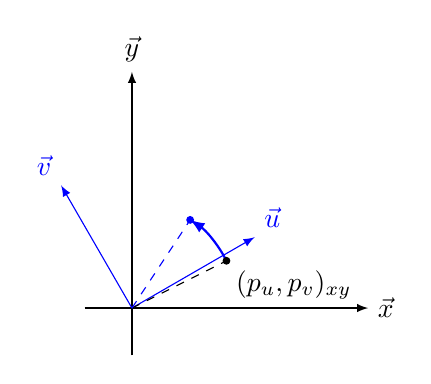
\begin{tikzpicture}[scale=0.6]
        \draw[-latex] (-1,0) -- (5,0) node[right] {$\vec{x}$};
        \draw[-latex] (0,-1) -- (0,5) node[above] {$\vec{y}$};
        \draw[-latex,blue] (0,0) -- (2.598,1.5) node[above right] {$\vec{u}$};
        \draw[-latex,blue] (0,0) -- (-1.5,2.598) node[above left] {$\vec{v}$};
        \draw[dashed] (0,0) -- (2,1);
        \draw[dashed,blue] (0,0) -- (1.232,1.866);
        \draw[-latex,blue,thick] (2,1) arc[start angle=26.565,end angle=56.565,radius=2.236];
        \filldraw[black] (2,1) circle (2pt) node[below right] {$(p_u,p_v)_{xy}$};
        \filldraw[blue] (1.232,1.866) circle (2pt);
    \end{tikzpicture}
}\subfigure{
    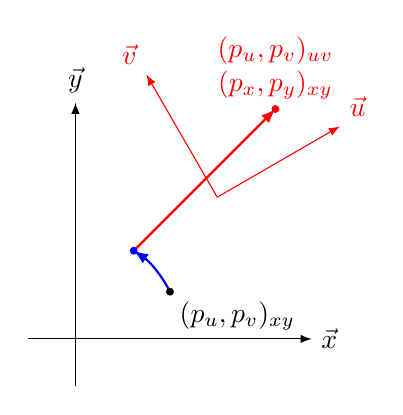
\begin{tikzpicture}[scale=0.6]
        \draw[-latex] (-1,0) -- (5,0) node[right] {$\vec{x}$};
        \draw[-latex] (0,-1) -- (0,5) node[above] {$\vec{y}$};
        \draw[-latex,blue,thick] (2,1) arc[start angle=26.565,end angle=56.565,radius=2.236];
        \draw[-latex,red,thick] (1.232,1.866) -- (4.232,4.866);
        \filldraw[blue] (1.232,1.866) circle (2pt);
        \draw[-latex,red] (3,3) -- (5.598,4.5) node[above right] {$\vec{u}$};
        \draw[-latex,red] (3,3) -- (1.5,5.598) node[above left] {$\vec{v}$};
        \filldraw[black] (2,1) circle (2pt) node[below right] {$(p_u,p_v)_{xy}$};
        \filldraw[red] (4.232,4.866) circle (2pt) node[above] {$(p_x,p_y)_{xy}$};
        \node[red,above] at (4.232,5.6) {$(p_u,p_v)_{uv}$};
    \end{tikzpicture}
}\caption{二维坐标系变换的示意图}
\end{figure}
\paragraph{三维坐标变换}
同样地,可以推出三维坐标系的矩阵表示为
\[\begin{bmatrix}
    p_x\\p_y\\p_z\\1
\end{bmatrix}=\begin{bmatrix}
    1&0&0&e_x\\
    0&1&0&e_y\\
    0&0&1&e_z\\
    0&0&0&1
\end{bmatrix}\begin{bmatrix}
    u_x&v_x&w_x&0\\
    u_y&v_y&w_y&0\\
    u_z&v_z&w_z&0\\
    0&0&0&1
\end{bmatrix}\begin{bmatrix}
    p_u\\p_v\\p_w\\1
\end{bmatrix}\]
\subsubsection{投影变换}
在解决坐标变换的问题后,我们需要将物体投影到观察平面上.这里我们介绍两种常见的投影方式:正交和透视投影.在此之前,需要明确一些投影中的概念.
\begin{definition}[投影线]
    连接对象点和投影点的直线称作\tbf{投影线}.
\end{definition}
\begin{definition}[平行投影]
    投影线相互平行的投影方式称作\tbf{平行投影}
\end{definition}
\begin{definition}[(投影)观察体]
    观察得到的图像对应在三维空间中的区域称作\tbf{(投影)观察体}.
\end{definition}
\begin{definition}[裁剪平面]
    观察体在$z$方向(也就是投影平面法向)的边缘通过选取平行于投影平面的两个平面决定,这两个平面分别称作\tbf{近裁剪平面}和\tbf{远裁剪平面},分别记作$z_{\text{near}}$和$z_{\text{far}}$.
\end{definition}
有时, $z_{\text{near}}$和$z_{\text{far}}$也指两个裁剪平面的$z$轴坐标.这需要依据上下文确定其含义.
\paragraph{正交投影}
我们先来介绍比较简单的投影方式.
\begin{definition}[正交投影]
    \tbf{正交投影}属于平行投影的一种,它的投影线全部与投影平面垂直.
\end{definition}
不难看出正交投影是保长度的,因此工程和建筑测绘常用正交投影.\\
\indent 正交投影从观察坐标到观察平面的变换很简单,任意一点$\vec{v}=(x,y,z)$的投影点就是$\vec{i}=(x,y)$.通常,需要将对象描述转化到规范化坐标系,即建立$\vec{v}\to[-1,1]^3$的映射(即将观察体映射到边长为$2$,范围从$(-1,-1,-1)$到$(1,1,1)$的立方体中).这对应于一个放缩操作,因此在齐次坐标系下正交投影的变换矩阵为
\[\mat{M}_{\text{ortho}}=\begin{bmatrix}
    \frac{2}{x_{\max}-x_{\min}}&0&0&-\frac{x_{\max}+x_{\min}}{x_{\max}-x_{\min}}\\
    0&\frac{2}{y_{\max}-y_{\min}}&0&-\frac{y_{\max}+y_{\min}}{y_{\max}-y_{\min}}\\
    0&0&\frac{2}{z_{\max}-z_{\min}}&-\frac{z_{\max}+z_{\min}}{z_{\max}-z_{\min}}\\
    0&0&0&1
\end{bmatrix}\]
其中$x_{\max},x_{\min},y_{\max},y_{\min}$分别为观察体在$x$和$y$方向上的上下界, $z_{\min}$和$z_{\max}$即为$z_{\text{near}}$和$z_{\text{far}}$.这样,在规范化坐标系中的坐标$(x',y',z')$和规范化前的坐标$(x,y,z)$就满足
\[\begin{bmatrix}
    x'&y'&z'&1
\end{bmatrix}^{\text{t}}=\mat{M}_{\text{ortho}}\begin{bmatrix}
    x&y&z&1
\end{bmatrix}^{\text{t}}\]
\paragraph{透视投影}
尽管正交投影容易生成,且可以保持对象的比例不变,但它的成像缺发真实感.人眼观察和相机拍摄到的图像通常符合透视投影规律.
\begin{definition}[透视投影]
    透视投影的投影线投影线汇聚于投影中心$C$,投影中心到投影平面的距离称为焦距,记作$f$.
\end{definition}
\indent 透视投影观察体是棱台形状,近剪切面$z_{\text{near}}$小,远剪切面$z_{\text{far}}$大.我们需要将观察体映射到一个适合正交投影的区域内(即将棱台映射到一个长方体内).具体而言,是把观察体挤压到一个以$z_{\text{near}}$为底面的长方体内.设观察体内一点$\vec{v}=(x,y,z)$变换到正交投影区域内的点$\vec{u}=\left(x',y',z'\right)$.根据相似三角形的性质,有
\[\dfrac{x'}{z_{\text{near}}}=\dfrac{x}{z},\quad\dfrac{y'}{z_{\text{near}}}=\dfrac{y}{z}\]
即
\[x'=\dfrac{xz_{\text{near}}}{z},\quad y'=\dfrac{yz_{\text{near}}}{z}\]
我们现在求矩阵$\mat{M}_{\text{persp}\to\text{ortho}}$使得在齐次坐标系下有
\[\begin{bmatrix}
    \vec{u}\\1
\end{bmatrix}=\mat{M}_{\text{persp}\to\text{ortho}}\begin{bmatrix}
    \vec{v}\\1
\end{bmatrix}\]
注意到$x',y'$的表达式中$z$在分母,这意味着映射可能是非线性的.为了避免这一情况,注意到对齐次坐标系的各个分量同乘一数不改变其含义,于是将两边同乘$z$可得(这里把$z$合并进矩阵中)
\[\begin{bmatrix}
    xz_{\text{near}}\\yz_{\text{near}}\\z'z\\z
\end{bmatrix}=\mat{M}_{\text{persp}\to\text{ortho}}\begin{bmatrix}
    x\\y\\z\\1
\end{bmatrix}\]
我们可以逆推出矩阵除第三行以外的形式.于是有
\[\begin{bmatrix}
    xz_{\text{near}}\\yz_{\text{near}}\\z'z\\z
\end{bmatrix}=\begin{bmatrix}
    z_{\text{near}}&0&0&0\\
    0&z_{\text{near}}&0&0\\
    m_{31}&m_{32}&m_{33}&m_{34}\\
    0&0&1&0
\end{bmatrix}\begin{bmatrix}
    x\\y\\z\\1
\end{bmatrix}\]
由于$z$坐标的变换与$x,y$坐标无关,因此$m_{31}=m_{32}=0$.自然,我们希望映射是线性的,不应该改变两个裁剪平面的$z$坐标值.于是分别将$z=z'=z_{\text{near}}$和$z=z'=z_{\text{far}}$代入矩阵的第三行可得
\[\left\{\begin{array}{l}
    z_{\text{near}}m_{33}+m_{34}=z_{\text{near}}^2\\
    z_{\text{far}}m_{33}+m_{34}=z_{\text{far}}^2
\end{array}\right.\]
解得$m_{33}=z_{\text{near}}+z_{\text{far}},m_{34}=-z_{\text{near}}z_{\text{far}}$.这样,观察体就被映射到一个以近裁剪平面为底面,$z$坐标取值为$\left[z_{\text{near}},z_{\text{far}}\right]$的长方体内.再对此长方体应用前面求出的正交投影的变换矩阵,可知投射投影的变换矩阵为
\[\begin{aligned}
    \mat{M}_{\text{persp}}
    &=\mat{M}_{\text{ortho}}\mat{M}_{\text{persp}\to\text{ortho}}\\
    &=\begin{bmatrix}
    \frac{2}{x_{\max}-x_{\min}}&0&0&-\frac{x_{\max}+x_{\min}}{x_{\max}-x_{\min}}\\
    0&\frac{2}{y_{\max}-y_{\min}}&0&-\frac{y_{\max}+y_{\min}}{y_{\max}-y_{\min}}\\
    0&0&\frac{2}{z_{\text{far}}-z_{\text{near}}}&-\frac{z_{\text{far}}+z_{\text{near}}}{z_{\text{far}}-z_{\text{near}}}\\
    0&0&0&1
    \end{bmatrix}\begin{bmatrix}
    z_{\text{near}}&0&0&0\\
    0&z_{\text{near}}&0&0\\
    0&0&z_{\text{near}}+z_{\text{far}}&-z_{\text{near}}z_{\text{far}}\\
    0&0&1&0
    \end{bmatrix}
\end{aligned}\]
这就完成了把观察体映射到规范化坐标系的立方体内的过程.\\
\indent 需要注意的是,在透视投影后的第四个分量即为深度值$z$,这在后续的深度测试中会用到.此外,根据齐次坐标的定义,在使用透视投影矩阵后需要再做一次齐次除法,即将前三个分量分别除以第四个分量,才能得到最终的规范化坐标系下的坐标值.
\paragraph{视口映射}
在完成将观察体映射到规范化坐标系的工作后,由于不同设备的屏幕分辨率大小不同,我们需要将规范化坐标系内的物体再映射到屏幕坐标上(这里不对$z$坐标做变换,在以后的步骤中另有他用).假定屏幕的宽度和高度分别为$w,h$,那么视口变换就是把$xy$坐标$[-1,1]\times[-1,1]$映射到$[0,w]\times[0,h]$上.这也是一个放缩操作,因此不难写出视口变换的矩阵为
\[\mat{M}_{\text{view}}=\begin{bmatrix}
    w/2&0&0&w/2\\
    0&h/2&0&h/2\\
    0&0&1&0\\
    0&0&0&1
\end{bmatrix}\]
\end{document}